\section{Schedule classification}

Classify the given schedule with respect to CSR (Conflict Serializable) and VSR (View Serializable) classes:
\[r_1(x) r_2(y) w_3(y) r_5(x) w_5(u) w_3(s)w_2(u) w_3(x) w_1(u) r_4(y) w_5(z) r_5(z)\]

\paragraph*{Solution}
To analyze the schedule, we first divide it based on the resources:
\begin{itemize}
    \item $x: r_1 \: r_5 \:w_3$
    \item $y: r_2 \: w_3 \:r_4$
    \item $z: w_5 \: r_5$
    \item $s: w_3$
    \item $u: w_5 \: w_2 \:w_1$
\end{itemize}
The conflict graph is constructed based on write-write or write-read relations in the resource groups. 
The nodes are $\{1,2,3,4,5\}$, and the arcs are determined by the conflicts. 
As a result we have the following graph:
\begin{figure}[H]
    \centering
    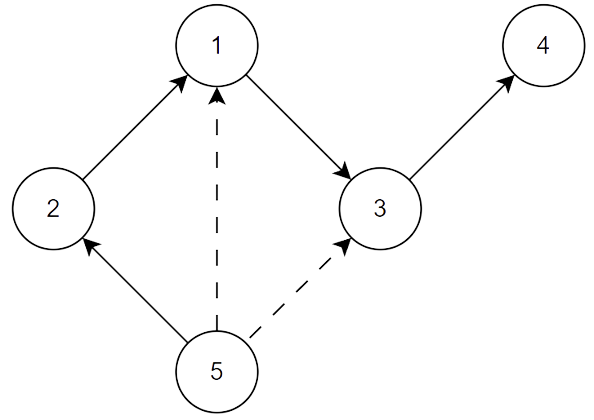
\includegraphics[width=0.5\linewidth]{images/conflictgraph.png}
\end{figure}
Some arcs can be omitted if the nodes are connected in another way (in this case, arcs $\{\{5,1\}$ and $\{5,3\}\}$ can be omitted).
Since there are no cycles in the graph, the schedule is both CSR and VSR.